\subsection{Background}

%\subsubsection{The Evolutionary Dungeon Designer} 
%Summarize EDD in its current status (what's described on the IEEE TOG paper).

%\subsubsection{Evolving Dungeons as a Whole, Room by Room}

% \begin{figure}[t]
% \centerline{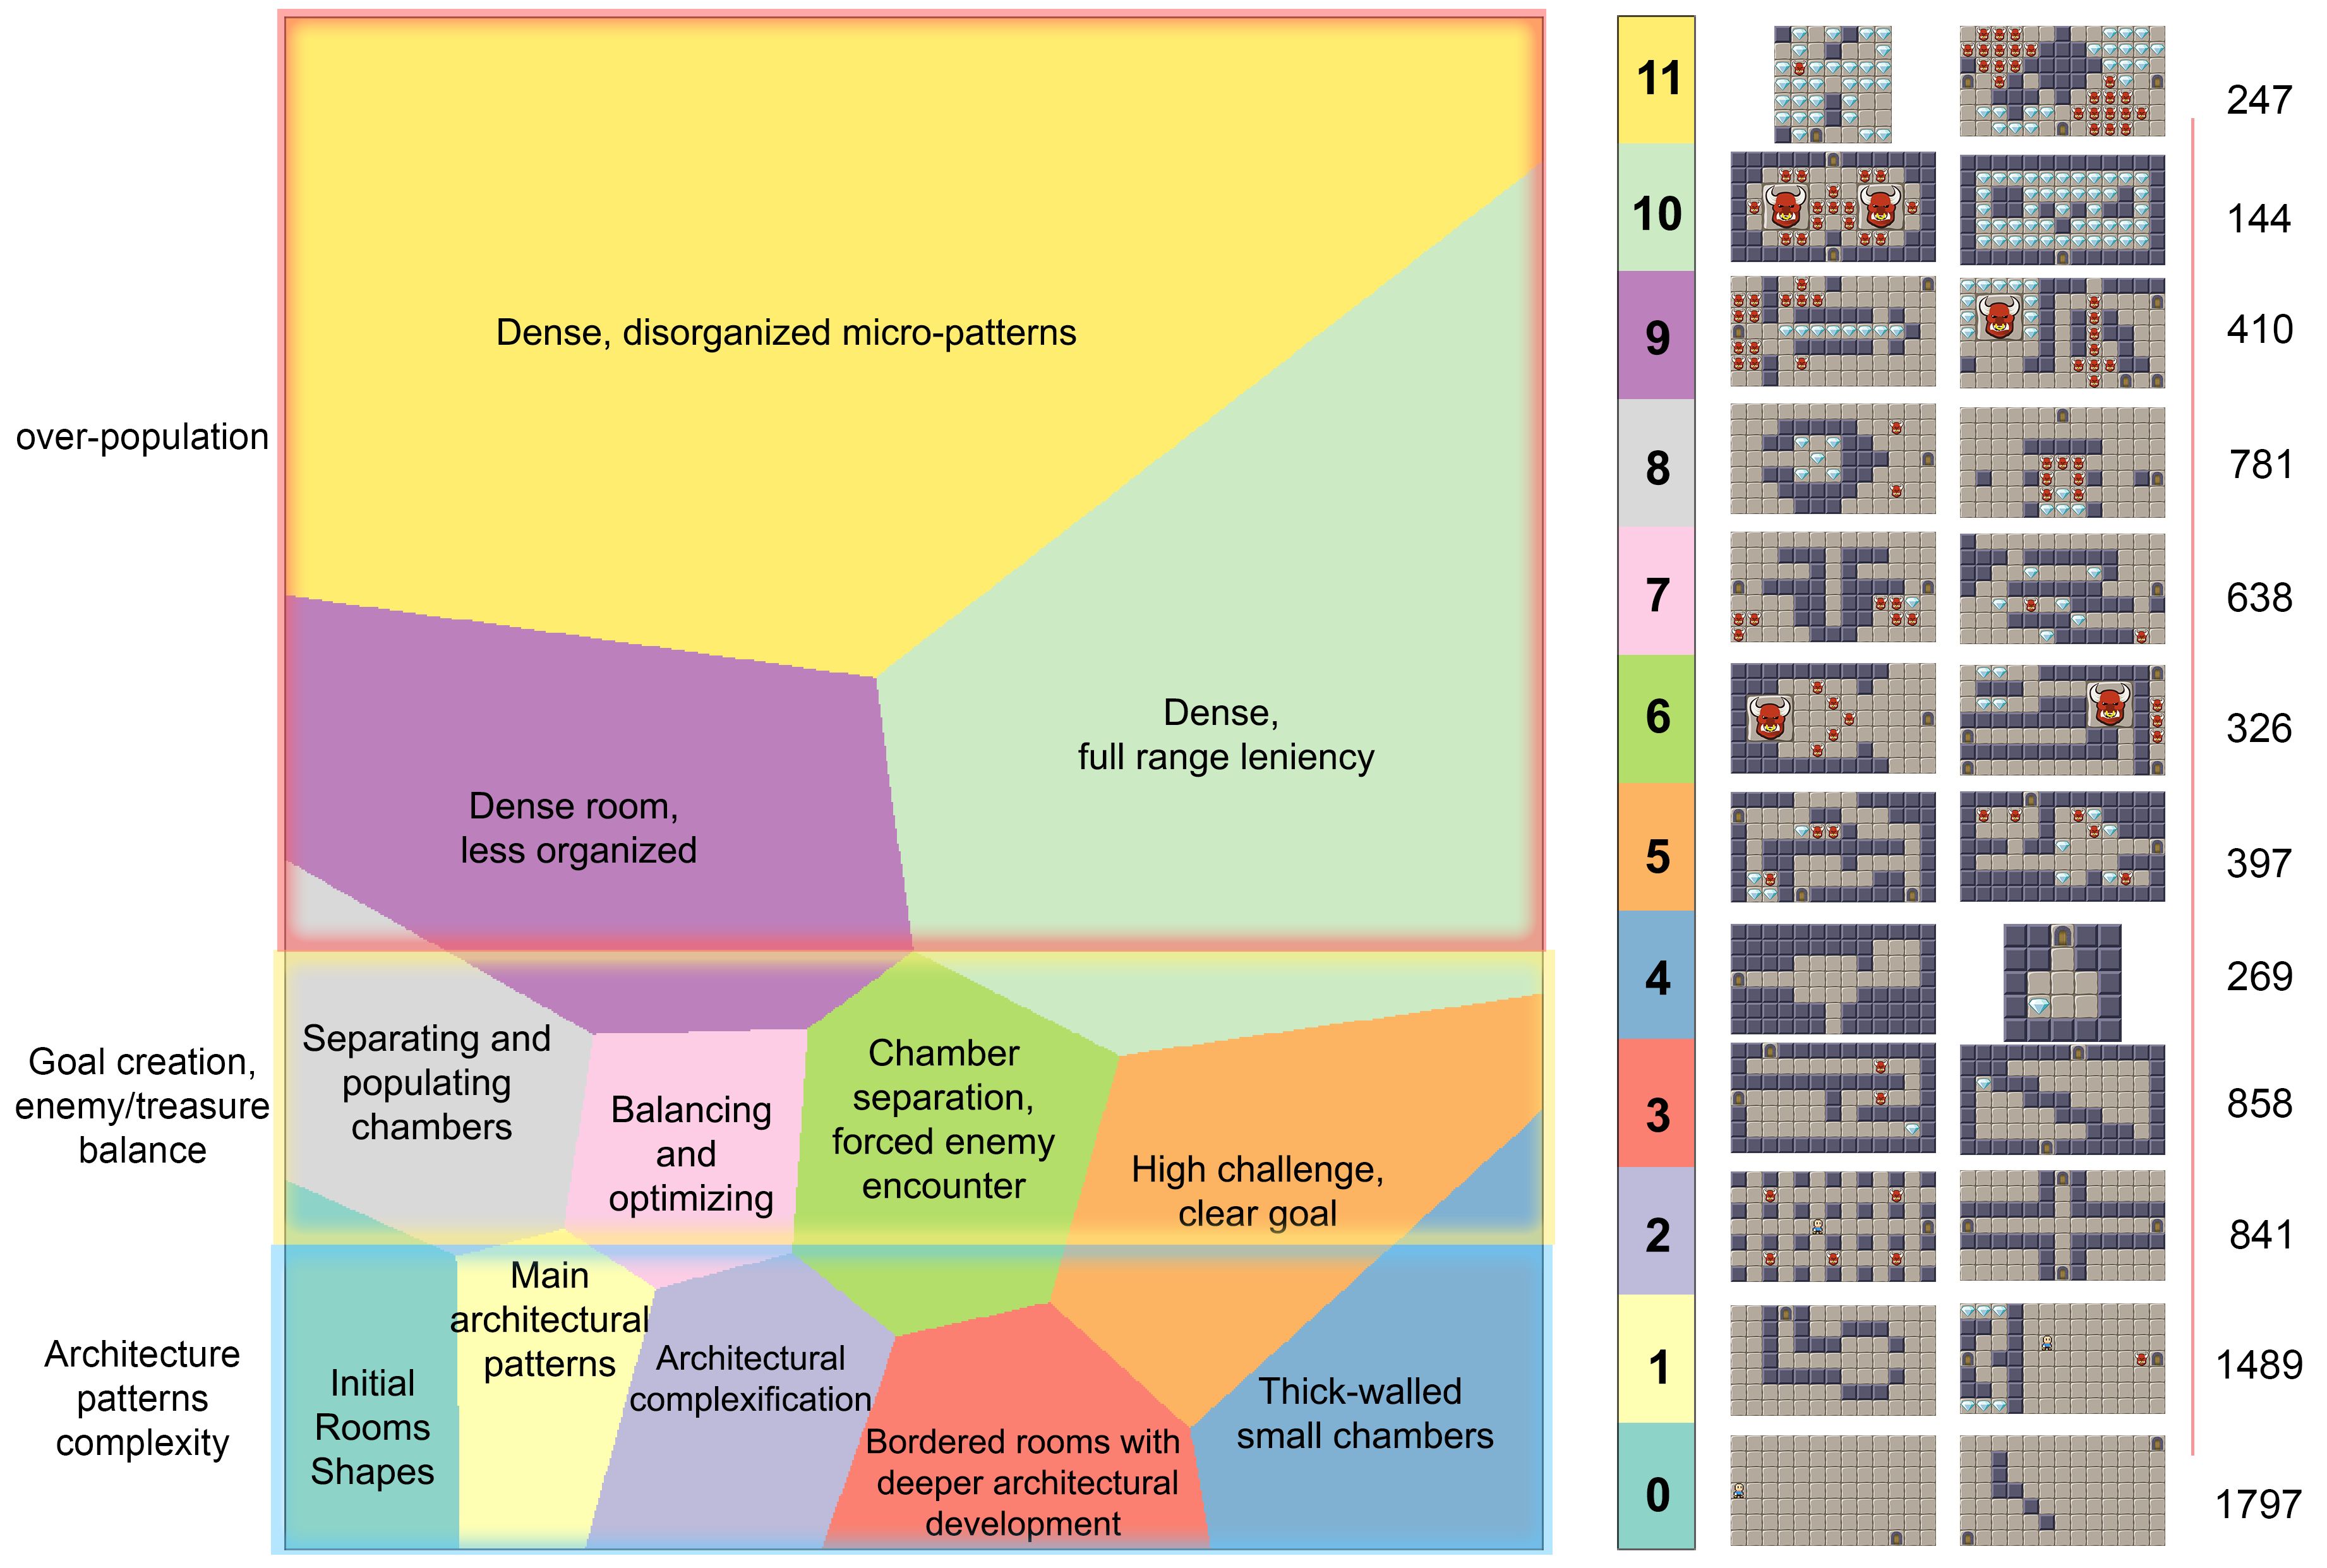
\includegraphics[width=9cm]{figures/figure2.png}}
% \caption{Screenshot of the dungeon editor screen in EDD, displaying a sample dungeon composed by seven rooms. The shortest path between two given tiles is highlighted in blue. The right pane contains all options for editing the dungeon. "M", "C", and "P" stand for "Move rooms", "Connect rooms", and "calculate Path".}
% \label{figs:dungeonscreen}
% \end{figure}
% \begin{figure}[t]
% \centerline{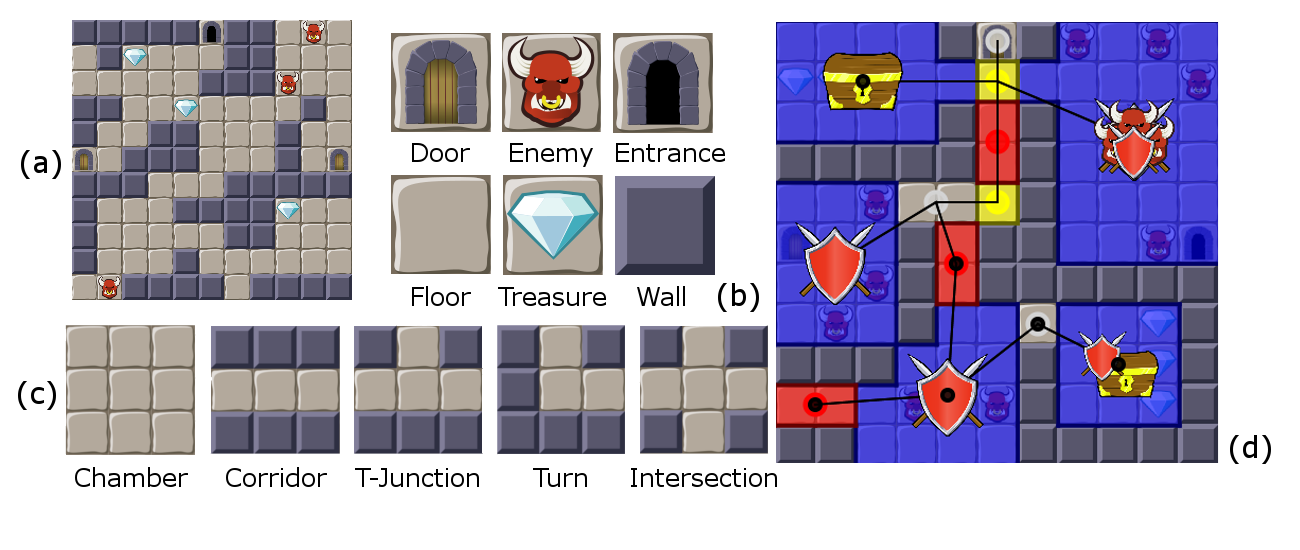
\includegraphics[width=9cm]{figures/figure1.png}}
% \caption{The EDD components. (a) A room, (b) placeable tiles, (c) micro- and (d) meso-patterns~\cite{p9Alvarez2018a}.}
% %\caption{The main components in EDD. (a) A basic room, (b) different placeable tiles, (c) micro-patterns and (d) meso-patterns~\cite{p9Alvarez2018a}.}
% \label{figs:basecomponents}
% \end{figure}


%The Evolutionary Dungeon Designer (EDD) is a Mixed-Initiative Co-Creativity (MI-CC) tool under continuous development. Its purpose is to allow a human designer create, or co-create with the AI, a 2D dungeon with rooms and corridors in the style of those appearing in the seminal game \emph{The Legend of Zelda}~\cite{p9tloz}.
The Evolutionary Dungeon Designer (EDD) is a MI-CC tool %under continuous development. It that allows 
to %create, or 
co-create 
%with the AI, 
2D dungeons in the style of the seminal game \emph{The Legend of Zelda}~\cite{p9tloz}.
%in the style of those appearing in the seminal game
% (\Cref{figs:basecomponents}.a).  The EDD workflow lets the 
Designers manually edit the dungeon structure as well as the interior of every room in it. EDD constantly offers tailored room suggestions on the fly that designers may decide to incorporate to their designs at any moment. 

In EDD, the system analyzes the level-design patterns (i.e., micro- and meso-patterns) that exist in each room, calculating and utilizing their quality to assess rooms. Micro-patterns are the building blocks in a design, which in EDD are categorized as \textit{spatial micro-patterns}: chamber, corridor, intersections, connector; and \textit{inventorial micro-patterns}: enemy, treasure, and door. On the other hand, Meso-patterns are defined as the relation between micro-patterns or other meso-patterns, and by the composition between inventorial micro-patterns and spatial micro-patterns. Meso-patterns are used to identify structures in the room that join together a set of micro-patterns and can be: \textit{ambush}, \textit{guard chamber}, \textit{treasure chamber}, and \textit{guarded treasure}. All patterns are shown in figure~\ref{fig:basecomponents}, and further information and discussion can be found in~\cite{p9Baldwin2017,Alvarez2018}.

\begin{figure}[b]
\centerline{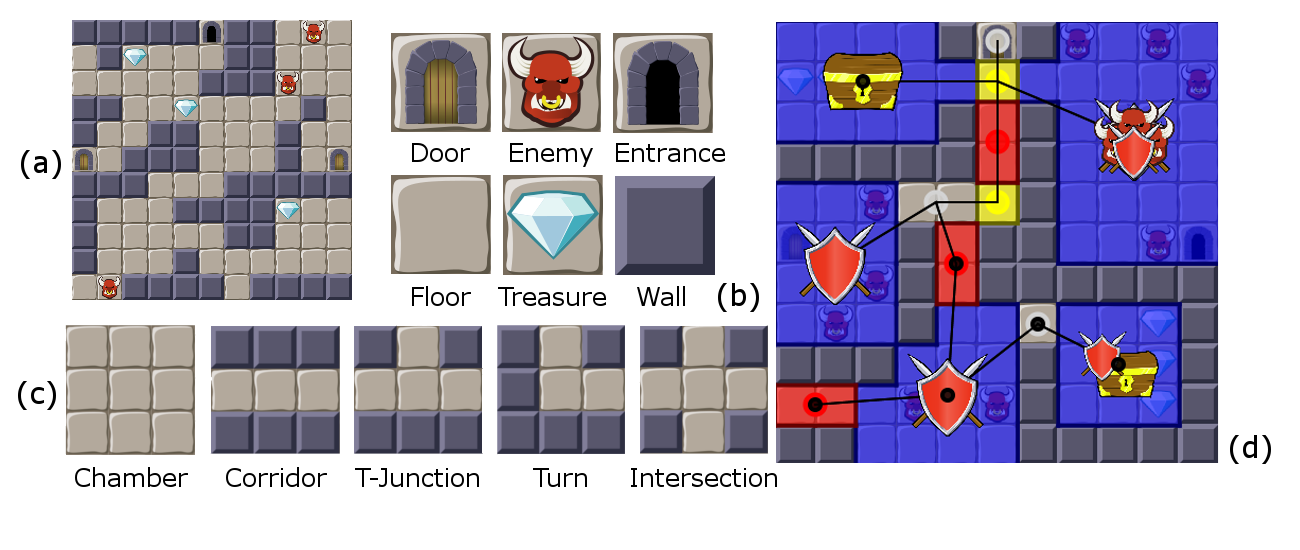
\includegraphics[width=9cm]{figures/figure1.png}}
\caption{Main components in EDD. (a) Basic room, (b) different tiles, (c) micro-patterns and (d) meso-patterns}
\label{fig:basecomponents}
\end{figure}


%to edit the dungeon by adding or removing rooms or by editing the rooms' tiles.
%The EDD workflow let the designer to manually edit the dungeon by adding or removing rooms or by editing the rooms' tiles.% (\Cref{figs:basecomponents}.b)  (\Cref{figs:basecomponents}.c and \Cref{figs:basecomponents}.d). A detailed description of all EDD's features, including the use of game design patterns, can be found in~\cite{p9Baldwin2017a, Baldwin2017, Alvarez2018, Alvarez2018a}. The foundation of the MI-CC approach in EDD is the use of EC aiming to find optimal candidates with game design patterns and design symmetry as objectives for the evolutionary search.

% An extensive description of EDD's features can be found throughout~\cite{p9Baldwin2017,Alvarez2018} %~\cite{p9Alvarez2018}

% as well as a complete description of its underlying %. The latest extension to EDD is the utilization of 
% IC MAP-Elites~\cite{p9Alvarez2020-ICMAPE}.
%With this function the designer can pick and choose from different procedurally generated room suggestions. With this function With this, the designer can choose from diverse room suggestions. The IC MAP-Elites are provided by continuous evolution and visually organized by dimensional customization.
%\begin{figure*}[t]
%\centerline{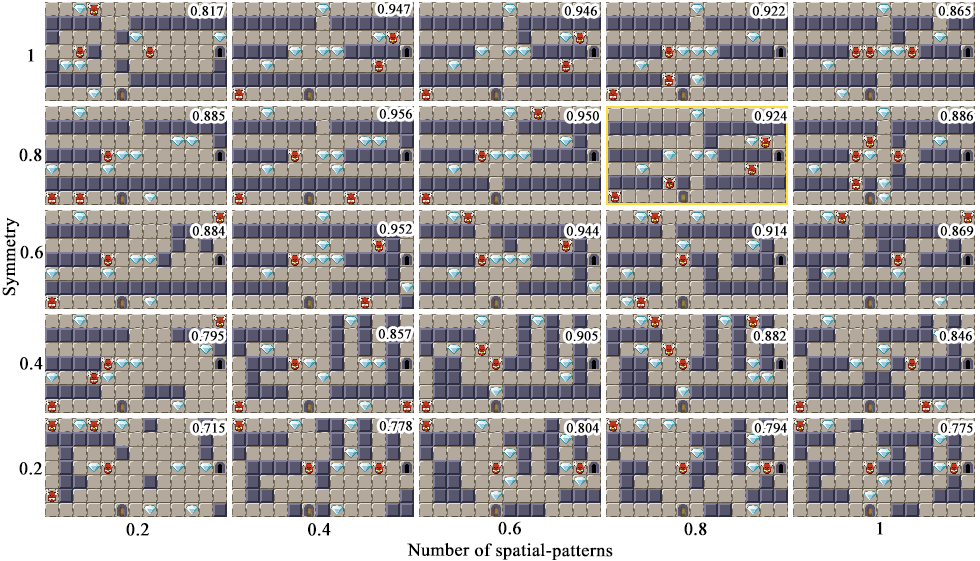
\includegraphics[width=13cm]{figures/figure3.jpg}}
%\caption{The room editor screen in EDD. The left pane contains all the options for manually editing the room displayed at the center-left of the screen. The right section displays the procedurally generated suggestions.}
%\label{figs:roomscreen}
%\end{figure*}
%In this section we present the latest version of EDD\footnote{Available for download at \url{https://github.com/mau-games/eddy}}, which includes significant improvements based on the outcomes from the qualitative analysis discussed in~\cite{p9Alvarez2018}. The most significant upgrade is replacing the grid-based backbone that represented the dungeon by a more flexible graph-based representation. A dungeon is now a graph of interconnected rooms of any given size between $3\times3$ and $20\times20$ tiles. The smallest allowed dungeon is composed by two rooms with one connection to each other. The designer can perform the following new actions: 
%\begin{itemize}
%\item adding disconnected rooms to the dungeon. Rooms may also be removed at any time.
%\item connecting any pair of rooms by adding a new bi-directional connection to the graph. Rooms interconnect from and to passable border tiles (self-loops are not allowed). Both ends are marked with a door tile (\Cref{figs:basecomponents}.b). A single border tile can only hold one connection, implying that a room can have as many connections as passable border tiles. Connections and rooms can be removed at any time, and their associated doors removed with them.% Removing a room also removes its connections.
%\item calculating paths between any pair of passable tiles located in any connected room. Paths are automatically calculated according to one of the following heuristics: \textit{fastest} returns the shortest path, \textit{rewarding} returns the path that traverses the highest number of treasure tiles, \textit{less danger} provides a path with the fewest number of enemies, whereas \textit{more danger} does the opposite. 
%\end{itemize}
%The designer is required to select one of the added rooms as the \textit{initial room}, which is the first room the player meets when entering the dungeon. This selection can be modified unlimited times. The \textit{initial room} is used by EDD to calculate the feasibility of the dungeon. A dungeon is considered feasible when there is at least one path between the \textit{initial room} and any other passable tile in every room. Rooms and doors that are unreachable from the \textit{initial room} are highlighted in red, so that they can be easily identified by the designer. This feasibility constraint ensures that all passable tiles are accessible, avoiding the possibility of accidentally creating unreachable areas.  
% \paragraph{The mixed-initiative workflow in EDD}
%The starting screen in EDD is the dungeon editor screen. Every new room is empty (composed solely of floor tiles) when created and is placed detached from the dungeon graph. After manually connecting the room to the dungeon with at least one connection, the designer has the option to populate the room using the room editor screen (\Cref{figs:roomscreen}). This screen can be reached in two different ways:

%\begin{enumerate}
%\item directly: by double-clicking or zooming in (by using the mouse wheel or by pinching on the touchpad) on the room. 
%\item indirectly: by clicking on the "Start with our suggestions" button, six procedurally generated suggestions are displayed on a separate screen. The selected suggestion is then opened in the room editor screen. 
%\end{enumerate}

%\Cref{figs:roomscreen} shows the room editor screen displaying a sample room with the dimensions $7\times5$ tiles. The left pane lists all the available options for manually editing the room. Manual editing is carried out by brush painting over the room with one of the available tile types: floor, wall, treasure, or enemy. There are two brush sizes (single tile and five-tile cross shape), and control-clicking allows the designer to bucket paint all adjacent tiles of the same type. Brush painting with the lock button on preserves selected tiles in all the procedurally generated suggestions. A detailed description of all the options in this pane is included in~\cite{p9Alvarez2018, Alvarez2018a}.

%The right side of the screen displays the procedurally generated suggestions, by means of the Interactive Constrained MAP-Elites genetic algorithm (see \Cref{section:3}).  
%When the designer accesses the room editor screen, the EA starts and continuously populates the suggestions pane with elites. The evolutionary process is fed with the manually edited room (i.e. target room), so that every change in the room affects the generated suggestions. By clicking on "Apply Suggestion", the manually edited room is replaced by the selected suggestion, thus affecting the upcoming procedural suggestions. "Restart" restarts the EA, and "Go To World Grid" takes the user back to the dungeon editor screen.

\subsubsection{Methods for Evaluating PCG}

%Over the last few years 
Recent research %In recent years a %small number of research initiatives have focused 
focuses on methods for evaluating procedural algorithms. The work in~\cite{p9Gravina2019-blendingNotionsDiversity} %the experimental set-up is a soft robots evolution task and covers:
evaluates fitness, offspring and selection for five MAP-elite methods, whereas %The results exhibit good effects by joining novelty and surprise in Quality Diverse (QD) algorithms. %The results demonstrates good effects by incorporating novelty and surprise in Quality Diverse (QD) algorithms. Another approach to optimise procedural generation has been explored by Cook et al.~\cite{p9Cook2016-SecondPaperDanesh} and Another approach to optimise procedural generation
\cite{p9Cook2016-SecondPaperDanesh} shows how users can improve the generator with the aid of automatic parameter tuning and, consequently, evaluates the effect that it has on the generator. The work is continued in~\cite{p9Cook2019:ParameterBasedEvaluation} where two analytical techniques, smoothness and co-dependence, were introduced to analyze the impact of a parameter change and its %following 
effect on a generative system; all integrated in Danesh~\cite{p9Cook2021-danesh}. Liapis et al.~\cite{p9Liapis2014-designerModelImpl} did a similar evaluation as the one in this paper, using artificial agents simulating designer's choices of suggestions to evaluate and display properties of their designer's model.%, in this case a cellular automata-based system. By doing so, it is possible to work with procedural generators more precisely. 
%By building on~\cite{p9Cook2016-SecondPaperDanesh} the work is continued in~\cite{p9Cook2019:ParameterBasedEvaluation} where two analytical techniques, smoothness and co-dependence, were introduced in order to help analyze the impact of a parameter change and its following effect on a generative system, in this case a cellular automata-based system. By doing so, it is possible to work with procedural generators more precisely. 

Previously suggested evaluation methods include a top-down approach~\cite{p9Smith:2010:Expressive-range,Horn2014-comparativePCG}, called the \emph{expressive range analysis} (ERA) which refers to the idea of exploring and visualizing the content space. % of potential content
%One important aspect is to understand how biased a generator is towards creating certain kinds of content. 
Summerville~\cite{p9summerville2018expanding} proposes %presents a number of 
techniques for visually assessing and analyzing procedural systems, with other means of visual assessment 
including analysis of generative space and individual procedural artefacts. %This approach is argued to suit procedural Machine Learning systems better.
% of the generative space
%systems including other means of
%This approach is argued to suit Machine Learning based procedural systems better.